%===============================================================================
% LaTeX sjabloon voor de bachelorproef toegepaste informatica aan HOGENT
% Meer info op https://github.com/HoGentTIN/bachproef-latex-sjabloon
%===============================================================================

\documentclass{bachproef-tin}

\usepackage{hogent-thesis-titlepage} % Titelpagina conform aan HOGENT huisstijl
\usepackage{listings}


\usepackage{color}
\definecolor{lightgray}{rgb}{.9,.9,.9}
\definecolor{darkgray}{rgb}{.4,.4,.4}
\definecolor{purple}{rgb}{0.65, 0.12, 0.82}
\definecolor{green}{rgb}{0,.6,0}
\lstdefinelanguage{JavaScript}{
	keywords={break, case, catch, continue, debugger, default, delete, do, else, false, finally, for, function, if, in, instanceof, new, null, return, switch, this, throw, true, try, typeof, var, void, while, with},
	morecomment=[l]{//},
	morecomment=[s]{/*}{*/},
	morestring=[b]',
	morestring=[b]",
    morestring=[b]`,
	ndkeywords={class, export, boolean, throw, implements, import, @Component},
	keywordstyle=\color{blue}\bfseries,
	ndkeywordstyle=\color{purple}\bfseries,
	identifierstyle=\color{black},
	commentstyle=\color{green}\ttfamily,
	stringstyle=\color{red}\ttfamily,
	sensitive=true
}

\lstset{
	language=JavaScript,
	backgroundcolor=\color{lightgray},
	extendedchars=true,
	basicstyle=\footnotesize\ttfamily,
	showstringspaces=false,
	showspaces=false,
	numbers=left,
	numberstyle=\footnotesize,
	numbersep=9pt,
	tabsize=2,
	breaklines=true,
	showtabs=false,
	captionpos=b
}

\usepackage{tikz}
\usetikzlibrary{shapes.multipart}

%%---------- Documenteigenschappen ---------------------------------------------
% TODO: Vul dit aan met je eigen info:

% De titel van het rapport/bachelorproef
\title{How the change detection strategy affects
    performance in Angular applications with
    high-frequency updates}

% Je eigen naam
\author{Thomas Duchatelet}

% De naam van je promotor (lector van de opleiding)
\promotor{Thomas Aelbrecht}

% De naam van je co-promotor. Als je promotor ook je opdrachtgever is en je
% dus ook inhoudelijk begeleidt (en enkel dan!), mag je dit leeg laten.
\copromotor{Bonnie Brennan}

% Indien je bachelorproef in opdracht van/in samenwerking met een bedrijf of
% externe organisatie geschreven is, geef je hier de naam. Zoniet laat je dit
% zoals het is.
\instelling{---}

% Academiejaar
\academiejaar{2020-2021}

% Examenperiode
%  - 1e semester = 1e examenperiode => 1
%  - 2e semester = 2e examenperiode => 2
%  - tweede zit  = 3e examenperiode => 3
\examenperiode{2}

%===============================================================================
% Inhoud document
%===============================================================================

\begin{document}

%---------- Taalselectie -------------------------------------------------------
% Als je je bachelorproef in het Engels schrijft, haal dan onderstaande regel
% uit commentaar. Let op: de tekst op de voorkaft blijft in het Nederlands, en
% dat is ook de bedoeling!

\selectlanguage{english}

%---------- Titelblad ----------------------------------------------------------
\inserttitlepage

%---------- Samenvatting, voorwoord --------------------------------------------
\usechapterimagefalse
%\input{voorwoord}
%\input{samenvatting}

%---------- Inhoudstafel -------------------------------------------------------
\pagestyle{empty} % Geen hoofding
\tableofcontents  % Voeg de inhoudstafel toe
\cleardoublepage  % Zorg dat volgende hoofstuk op een oneven pagina begint
\pagestyle{fancy} % Zet hoofding opnieuw aan

%---------- Lijst figuren, afkortingen, ... ------------------------------------

% Indien gewenst kan je hier een lijst van figuren/tabellen opgeven. Geef in
% dat geval je figuren/tabellen altijd een korte beschrijving:
%
%  \caption[korte beschrijving]{uitgebreide beschrijving}
%
% De korte beschrijving wordt gebruikt voor deze lijst, de uitgebreide staat bij
% de figuur of tabel zelf.

\listoffigures
\listoftables

% Als je een lijst van afkortingen of termen wil toevoegen, dan hoort die
% hier thuis. Gebruik bijvoorbeeld de ``glossaries'' package.
% https://www.overleaf.com/learn/latex/Glossaries

%---------- Kern ---------------------------------------------------------------

% De eerste hoofdstukken van een bachelorproef zijn meestal een inleiding op
% het onderwerp, literatuurstudie en verantwoording methodologie.
% Aarzel niet om een meer beschrijvende titel aan deze hoofstukken te geven of
% om bijvoorbeeld de inleiding en/of stand van zaken over meerdere hoofdstukken
% te verspreiden!

\input{inleiding}
\chapter{\IfLanguageName{dutch}{Stand van zaken}{State of the art}}
\label{ch:stand-van-zaken}

% Tip: Begin elk hoofdstuk met een paragraaf inleiding die beschrijft hoe
% dit hoofdstuk past binnen het geheel van de bachelorproef. Geef in het
% bijzonder aan wat de link is met het vorige en volgende hoofdstuk.

% Pas na deze inleidende paragraaf komt de eerste sectiehoofding.

\section{What is a Front-end framework?}

A front-end framework is a paradigm of best practices and provides a certain approach to develop the front-end of an application.
Lots of webapplications share the same base features. A framework bundles these features and provides tool to easily develop them in a structured way. Web frameworks help us achieve structure in our applications and give developers a place to start and therefore leads to accelerated development. By defining several rules and best practices, a codebase is easier to understand for other developers when they have knowledge of the framework. \autocite{Spittel}

\section{Multiple-page vs single-page applications}

The classic approach of multiple-page applications (MPA) has the following flow:
\begin{enumerate}
    \item A user performs an action
    \item The client sends a request to the server
    \item The server consumes the action
    \item The server sends a new page to the client
    \item The client reloads the page
\end{enumerate}
With this approach the client always gets new pages and causes a reload on every user action.
When using a sngle-page application (SPA), the client downloads the application at first and the rendering happens on the client side. This way the page does not need a refresh on every user action. Though the client still communicates with the server for data, not for handling pages.
Given this we can state that an MPA uses server side rendering, while an SPA renders on the client side.
\autocite{Skolski}

\section{What is Angular?}
\subsection{Definition}
Angular is a platform and framework for building single-page client applications using HTML and TypeScript developed and maintained by developers at Google.
\autocite{Angular.io}

\subsection{AngularJs}
\subsubsection{Model-View-Whatever}
In October 2010 AngularJs first appeared on GitHub as an in-beta project. The framework became open-sourced and maintained by Google the following year. In June 2012 Google launched version 1.0 of AngularJs. \autocite{Brandrick2017} AngularJs used the Model-View-Controller architecture. This exists out of three layers: the model who defines the business rules, the view who is the user interface and the controller who switches data back and forth between the model and the view.
\autocite{AltexSoft}

\begin{figure}[h!]
    \caption{Model-View-Controller}
    \centering
    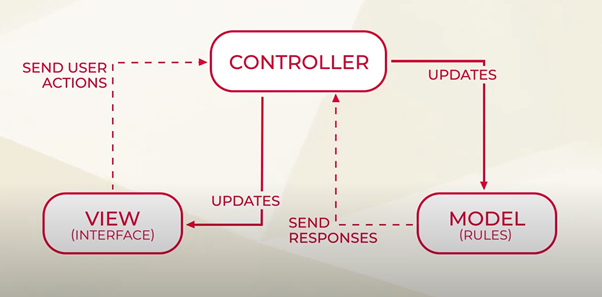
\includegraphics[width=\textwidth]{img/mvc.png} 
\end{figure}

AngularJs has two-way databinding to ease this process. With two-way databinding the model and the view are synchronized. Changes in the model are displayed on the view and vice versa. This means that developers do not have to write code for this purpose, the framework takes care of it. Therefore, the Angular team also defines it's architecture as Model-View-Whatever.

\autocite{Rauh}

\begin{figure}[h!]
    \caption{Two-way databinding}
    \centering
    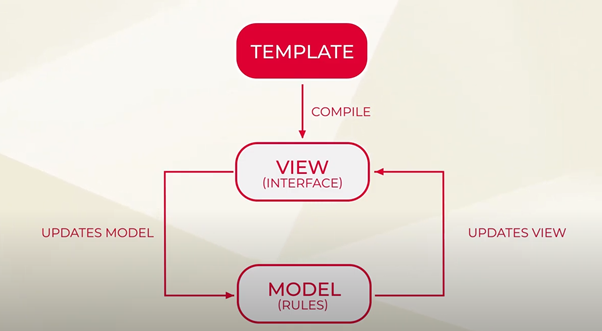
\includegraphics[width=\textwidth]{img/twowaydata.png} 
\end{figure}



\subsubsection{Dependency injection}
Another strength of AngularJs is dependency injection. An application traditionaly exists of different pieces of code that are related to each other.  Instead of attaching dependencies to objects, injectors are used that link these objects to dependencies stored in a central place. This improves the possibility for writing reusable code and isolated unit testing. \autocite{AltexSoft} This way dependency injection allows high cohesion and loose coupling between pieces of code. \autocite{Sterkowitz}


\subsubsection{Directives}
Further AngularJs provided directives as a popular feature. With directives it is possible to add behaviour to a HTML element which allows creating dynamic content. \autocite{AngularJs}

\subsubsection{Downside}
This set of features made AngularJs a good tool for creating SPA's. Though the framework opened a lot of possibilities, it suffered from performance issues when creating large SPA's. One of AngularJs' competitors, React, rolled back to one-way databinding and introduced components to deal with this issue. \autocite{AltexSoft}
\begin{figure}[h!]
    \caption{One-way databinding}
    \centering
    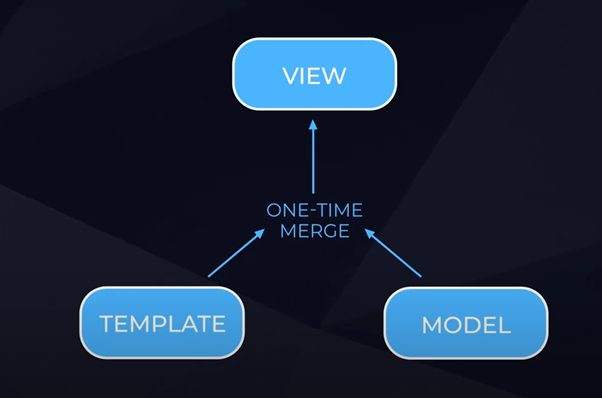
\includegraphics[width=\textwidth]{img/onewaydata.png} 
\end{figure}

\subsection{Angular}
\subsubsection{The update}
The rising popularity of React required the AngularJs team to improve. In September 2016 Google released Angular 2. For now every version starting from Angular 2 is referred to as Angular. AngularJs is every version beneath Angular 2. The reason this naming is important is because of the breaking changes Angular 2 introduced. It is not possible to automatically update AngularJs to Angular and the migrations require a lot of rework.
\autocite{Semenas2020}

\subsubsection{Improved databinding}
In response to the one-way databinding React used, Angular lets the developer define the communication between the component and it's template. The supported types of databinding are:
\begin{itemize}
    \item One-way
    \item Two-way
    \item Event
    \item Property
\end{itemize}
\autocite{AltexSoft}
\subsubsection{Modules and components}
One of the key principles of Angular is the division of an application in modules and components.
Angular is component based like React. The introduction of hierarchical components was a welcome change to deal with the performance issues and it improved code reusability as well. A component traditionally lives in a module, though with newer versions it is also possible to create stand-alone components which is still an experimental feature.
Every Angular application has a root module which takes care of the application startup. An application typically contains a set of feature modules and a shared module. Angular modules can import functionality from and export functionality to other modules. With a shared module it is possible to let feature modules not depend on each other. Organizing the application into distinct modules helps in designing for reusability. The division in modules also takes advantage of lazy-loading, this means only loading a module when it is needed, so the amount of code that needs to be loaded at startup is minimized. 
\autocite{Angular.io}

\begin{figure}[h!]
    \caption{Angular component structure}
    \centering
    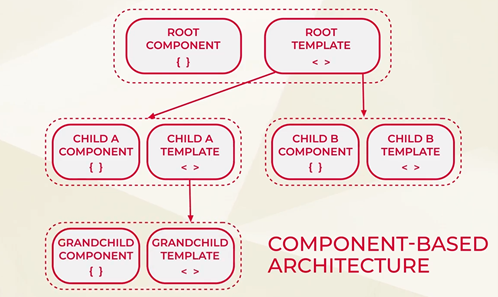
\includegraphics[width=\textwidth]{img/angularcomponent.png} 
\end{figure}

\subsubsection{State management}
Additionally Angular contains a useful library called NgRx that functions as a state and data management tool. In Angular each component has one state and no idea of other component's states. NgRx allows to share this state by keeping it in a single store. This principle is also called the single source of truth.
\autocite{AltexSoft}
\begin{figure}[h!]
    \caption{NgRx mechanism}
    \centering
    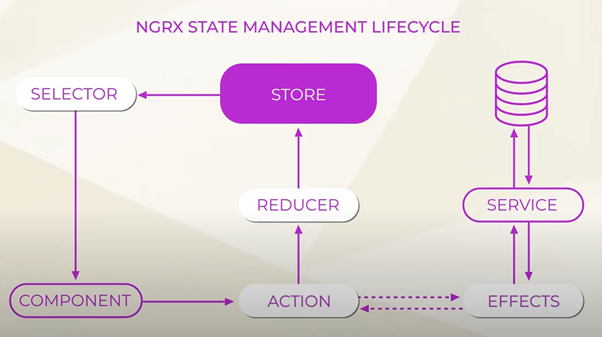
\includegraphics[width=\textwidth]{img/ngrx.png} 
\end{figure}

\subsubsection{Automatic change detection}
Moreover Angular uses Zone.Js to provide automatic change detection. When a model's state has changed, the Angular change detection updates the view to ensure the user interface is synchronized with the latest state of the model.
\autocite{Kumar2020}

\subsubsection{Typescript}
Another important change was that Angular now used Typescript instead of Javascript. Typescript provides static typing which makes it easier for developers to find mistakes before production and use Intellisense to speed up the development process. Typescript is also easy to read for developers with knowledge of Javascript and supports Javascript libraries. In fact, it assembles back to Javascript when compiling.
\autocite{Typescriptlang}

\subsubsection{Hierarchical dependency injection}
One more advantage over AngularJs is that dependency injection became hierarchical. A hierarchical dependency injection system allows to define different scopes for dependencies to run in and follows the component tree structure. This allows to create services that are not application wide but isolated to a subset of components.
\autocite{Rylan}
\begin{figure}[h!]
    \caption{Hierarchical dependency injection}
    \centering
    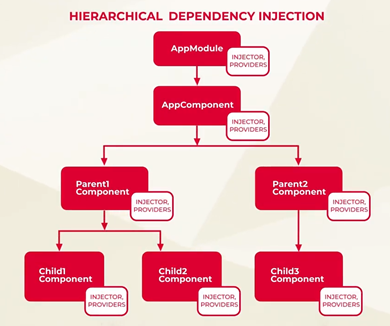
\includegraphics[width=\textwidth]{img/hieradi.png} 
\end{figure}

\subsubsection{Downside}
Many beginners will define Angular as a complex framework to start with. The framework contains lots of features and possibilities. This causes a steep learning curve. The Angular team provides continuous support and new features regularly which is welcomed by experienced developers on the one hand but makes the learning process more difficult for beginners on the other hand.
\autocite{AltexSoft}

\section{Change detection strategies in Angular}
\subsection{Default}
By default, Angular uses Zone.js to trigger change detection. Zone.js does not detect changes itself, instead the responsibility of Zone.js is notifying Angular when to run change detection. \autocite{Inatomi2020} The Angular change detection mechanism then loops over the component tree (starting from the top) to check for changes.
\begin{figure}[h!]
    \caption{Default change detection mechanism}
    \centering
    \includegraphics[width=.49\textwidth]{img/cycle1.png} 
    \includegraphics[width=.49\textwidth]{img/cycle2.png} 
    \includegraphics[width=.49\textwidth]{img/cycle3.png} 
    \includegraphics[width=.49\textwidth]{img/cycle4.png} 
\end{figure}

\subsection{OnPush}
With the \emph{OnPush} strategy it is possible to skip components when checking the component tree for changes. When \emph{OnPush} is used, the mechanism follows these steps:
\begin{enumerate}
    \item An event triggers the change detection.
    \item Change detection checks the component tree top to bottom, but skips the parts where \emph{OnPush} is used.
    \autocite{Hoffmann2019}
\end{enumerate}

\begin{figure}[h!]
    \caption{OnPush change detection mechanism}
    \centering
    \includegraphics[width=.49\textwidth]{img/onpush-cycle1.png} 
    \includegraphics[width=.49\textwidth]{img/onpush-cycle2.png} 
    \includegraphics[width=.49\textwidth]{img/onpush-cycle3.png} 
    \includegraphics[width=.49\textwidth]{img/onpush-cycle4.png} 
\end{figure}

Thanks to the custom strategy implemented by the developer, Angular will not update the components where \emph{OnPush} is defined unless:
\begin{itemize}
    \item The reference of an \emph{@Input} property changes.
    \item An event handler is triggered in the component or one of its children.
    \item An observable that uses the \emph{async} pipe in the template provides a new value.
    \item The change detection is triggered by the developer.
\end{itemize}
\subsection{Zoneless}

\section{Angular Ivy}
\subsection{Definition}
According to \textcite{Angular.io-ivy} is Ivy the code name for Angular's next-generation compilation and rendering pipeline. With the version 9 release of Angular, the new compiler and runtime instructions are used by default instead of the older compiler and runtime, known as View Engine.

\subsection{Compiler}
The Angular framework is a compiler. A component is written in Typescript and it's template is written in HTML with some additional Angular syntax (directives). When building, Angular compiles this code to a set of Javascript instructions who are able to create and modify the DOM when a component is rendered on the page. If Angular was a car, the compiler would be the engine.

\subsection{Most important features}
The release of Ivy opens up a lot of new potential features. Most of these features are still experimental as the Angular does not want to introduce breaking changes with the new update. Experimental methods are marked with the Greek letter \(\Theta\) (Theta) so developers know this could cause issues when updating. The most important features of Angular Ivy are:
\begin{itemize}
    \item Better build times by ahead-of-time (AOT) compilation
    \item Smaller bundle size by improved tree-shaking
    \item Metaprogramming by using higher order components \autocite{Savkin2018}
    \item Lazy loading of components by using stand-alone components
    \item New change detection system without Zone.js
    \item Ease the publishing process of libraries to NPM
\end{itemize}

\autocite{Exbrayat2019}


\section{RxJs}

\section{Typescript Decorators}

\section{SignalR}

%%=============================================================================
%% Methodologie
%%=============================================================================

\chapter{\IfLanguageName{dutch}{Methodologie}{Methodology}}
\label{ch:methodologie}

%% TODO: Hoe ben je te werk gegaan? Verdeel je onderzoek in grote fasen, en
%% licht in elke fase toe welke stappen je gevolgd hebt. Verantwoord waarom je
%% op deze manier te werk gegaan bent. Je moet kunnen aantonen dat je de best
%% mogelijke manier toegepast hebt om een antwoord te vinden op de
%% onderzoeksvraag.

\section{Introduction}
To be able to measure the differences in performance, three applications will be developed. All applications will recieve SignalR updates from the server and draw twenty real-time charts in the browser and animate the updated data. The first application will let Zone.js and default Angular change detection handle everything. In the second application the changeDetectorRef will be injected and the onPush strategy will be used to achieve the same goal. In the third application, Zone.js will be excluded from the project and the Angular Ivy internal private API will be used to handle change detection fully manual. Afterwards the performance of all three applications can be measured and compared.

\section{Default change detection application}
First of all, a new application should be created. This can be done by running following command in the terminal.
\begin{lstlisting}[language=bash]
$ ng new default
\end{lstlisting}

Now the terminal should navigate to the app directory into the newly generated project folder.

\begin{lstlisting}[language=bash]
	$ cd default/src/app
\end{lstlisting}

In the app directory, a new module should be created to hold all components regarding the dashboard with the charts. This way lazy loading could be used when the application would be extended with additional functionality that doesn't require the charting library.

\begin{lstlisting}[language=bash]
	$ ng g m dashboard
\end{lstlisting}

This command creates a folder with a dashboard module. Now the terminal can navigate to this folder using:

\begin{lstlisting}[language=bash]
	$ cd dashboard
\end{lstlisting}

In the dashboard folder, a dashboard component can be generated which will hold all the charts.

\begin{lstlisting}[language=bash]
	$ ng g c dashboard
\end{lstlisting}

To keep an overview of all files, some additional folders are a good practice. Therefore two more folders shall be created to hold the models and services.

\begin{lstlisting}[language=bash]
	$ mkdir models
	$ mkdir services
\end{lstlisting}

The dashboard component will need some configuration data to know how to draw the charts. This could be hardcoded but since it is likable to maintain flexibility in the application, the configuration will be stored in an object. To create the class for this object, the terminal should move to the models folder and generate the class. An additional enum will also be generated to hold the possible types of charts the application supports.

\begin{lstlisting}[language=bash]
	$ cd models
	$ ng g class ChartSetting
	$ ng g enum ChartType
\end{lstlisting}

Then the types of supported charts are defined in the enum.

\begin{lstlisting}[language=JavaScript]
	export enum ChartType {
		Line = 0,
		Bar = 1,
		Scatter = 2,
		Pie = 3
	}
\end{lstlisting}

Now the chart settings model can be build. To start, this contains a title and a type but can be extended in the future when needed.

\begin{lstlisting}[language=JavaScript]
	import { ChartType } from "./chart-type.enum";
	
	export class ChartSetting {
		title: string;
		type: ChartType;
	}
\end{lstlisting}

To fetch the chart configuration containing the data the dashoard component needs to draw the charts on the dashboard, a service is a good solution because it allows reuse of code.
 
\begin{lstlisting}[language=bash]
	$ cd ../services
	$ ng g s chartSettings
\end{lstlisting}

This service could make an API call if the charts should be configurable, but for now a static area of twenty charts is returned. Notice the @Injectable statement above the class declaration. This enables to inject the service in the constructor of a component.

\begin{lstlisting}[language=JavaScript]
	import { Injectable } from '@angular/core';
	import { ChartSetting } from '../models/chart-setting';
	import { ChartType } from '../models/chart-type.enum';
	
	@Injectable({
		providedIn: 'root'
	})
	export class ChartSettingsService {
		
		constructor() { }
		
		get chartSettings(): ChartSetting[]{
			return [
				{title: 'line1', type: ChartType.Line},
				{title: 'line2', type: ChartType.Line},
				{title: 'line3', type: ChartType.Line},
				{title: 'line4', type: ChartType.Line},
				{title: 'line5', type: ChartType.Line},
				{title: 'Bar1', type: ChartType.Bar},
				{title: 'Bar2', type: ChartType.Bar},
				{title: 'Bar3', type: ChartType.Bar},
				{title: 'Bar4', type: ChartType.Bar},
				{title: 'Bar5', type: ChartType.Bar},
				{title: 'Scatter1', type: ChartType.Scatter},
				{title: 'Scatter2', type: ChartType.Scatter},
				{title: 'Scatter3', type: ChartType.Scatter},
				{title: 'Scatter4', type: ChartType.Scatter},
				{title: 'Scatter5', type: ChartType.Scatter},
				{title: 'Pie1', type: ChartType.Pie},
				{title: 'Pie2', type: ChartType.Pie},
				{title: 'Pie3', type: ChartType.Pie},
				{title: 'Pie4', type: ChartType.Pie},
				{title: 'Pie5', type: ChartType.Pie}
			];
		}
	}
\end{lstlisting}

The next step is to create a component for each type of chart that holds the logic for drawing the chart. To stick to the DRY (Don't Repeat Yourself) pattern, an additional BaseChart component will be created that will hold the logic for listening to SignalR later on.

\begin{lstlisting}[language=bash]
	$ cd ..
	$ mkdir charts
	$ cd charts
	$ ng g c baseChart
	$ ng g c lineChart
	$ ng g c barChart
	$ ng g c scatterChart
	$ ng g c pieChart
\end{lstlisting}

In the BaseChart component an Input property should be added so the dashboard can pass the configuration to its child component.

\begin{lstlisting}[language=JavaScript]
	export class BaseChartComponent implements OnInit {
		@Input() chartSettings: ChartSetting;
		...
	}
\end{lstlisting}

The other chart components should inerit from the BaseChart component so they can access the chart settings as well.

\begin{lstlisting}[language=JavaScript]
	export class LineChartComponent extends BaseChartComponent implements OnInit {
		constructor() {
			super();
		}
		...
	}

	export class BarChartComponent extends BaseChartComponent implements OnInit {
		constructor() {
			super();
		}
		...
	}
	
	export class ScatterChartComponent extends BaseChartComponent implements OnInit {
		constructor() {
			super();
		}
		...
	}
	
	export class PieChartComponent extends BaseChartComponent implements OnInit {
		constructor() {
			super();
		}
		...
	}
\end{lstlisting}

Now this is set up, the ChartSettings service has to be injected in the constructor of the dashboard component and passed on to the chart components. The dashboard component will look as following:
 
\begin{lstlisting}[language=JavaScript] 	
 	@Component({
 		selector: 'app-dashboard',
 		templateUrl: './dashboard.component.html',
 		styleUrls: ['./dashboard.component.css']
 	})
 	export class DashboardComponent implements OnInit {
 		chartSettings: ChartSetting[] = [];
 		
 		constructor(private _chartSettingsService: ChartSettingsService) { }
 		
 		ngOnInit() {
 			this.chartSettings = this._chartSettingsService.chartSettings;
 		}
 	
	 	// This is a trick to expose the enum to the view so no magic numbers are needed
	 	get chartTypes(): typeof ChartType {
	 		return ChartType;
	 	}	
 	}
\end{lstlisting}

The HTML template will loop over the settings, check the type and render the right component for each type.

 
\begin{lstlisting}[language=JavaScript] 	
	<div *ngFor='let setting of chartSettings'>
		<div *ngIf='setting.type === chartTypes.Line'>
			<app-line-chart [chartSettings]='setting'></app-line-chart>
		</div>
		<div *ngIf='setting.type === chartTypes.Bar'>
			<app-bar-chart [chartSettings]='setting'></app-bar-chart>
		</div>
		<div *ngIf='setting.type === chartTypes.Scatter'>
			<app-scatter-chart [chartSettings]='setting'></app-scatter-chart>
		</div>
		<div *ngIf='setting.type === chartTypes.Pie'>
			<app-pie-chart [chartSettings]='setting'></app-pie-chart>
		</div>
	</div>
	
\end{lstlisting}

If the app is served, still nothing shows up in the browser. This is because Angular bootstraps the app component but the new dashboard component is not imported yet. If the dashboard module is imported in the browser, some text is displayed which state that the chart components work.










% Voeg hier je eigen hoofdstukken toe die de ``corpus'' van je bachelorproef
% vormen. De structuur en titels hangen af van je eigen onderzoek. Je kan bv.
% elke fase in je onderzoek in een apart hoofdstuk bespreken.

%%=============================================================================
%% Default change detection strategy
%%=============================================================================

\chapter{\IfLanguageName{dutch}{Default change detection strategy}{Default change detection strategy}}
\label{ch:default}

This chapter describes the steps that were followed to create the first Angular application with a default change detection strategy.

First of all, a new application should be created. This can be done by running following command in the terminal.
\begin{lstlisting}[language=bash]
$ ng new default
\end{lstlisting}

Now the terminal should navigate to the app directory into the newly generated project folder.

\begin{lstlisting}[language=bash]
	$ cd default/src/app
\end{lstlisting}

In the app directory, a new module should be created to hold all components regarding the dashboard with the charts. This way lazy loading could be used when the application would be extended with additional functionality that doesn't require the charting library.

\begin{lstlisting}[language=bash]
	$ ng g m dashboard
\end{lstlisting}

This command creates a folder with a dashboard module. Now the terminal can navigate to this folder using:

\begin{lstlisting}[language=bash]
	$ cd dashboard
\end{lstlisting}

In the dashboard folder, a dashboard component can be generated which will hold all the charts.

\begin{lstlisting}[language=bash]
	$ ng g c dashboard
\end{lstlisting}

To keep an overview of all files, some additional folders are a good practice. Therefore two more folders shall be created to hold the models and services.

\begin{lstlisting}[language=bash]
	$ mkdir models
	$ mkdir services
\end{lstlisting}

The dashboard component will need some configuration data to know how to draw the charts. This could be hardcoded but since it is likable to maintain flexibility in the application, the configuration will be stored in an object. To create the class for this object, the terminal should move to the models folder and generate the class. An additional enum will also be generated to hold the possible types of charts the application supports.

\begin{lstlisting}[language=bash]
	$ cd models
	$ ng g class ChartSetting
	$ ng g enum ChartType
\end{lstlisting}

Then the types of supported charts are defined in the enum.

\begin{lstlisting}[language=JavaScript]
	export enum ChartType {
		Line = 0,
		Bar = 1,
		Scatter = 2,
		Pie = 3
	}
\end{lstlisting}

Now the chart settings model can be build. To start, this contains a title and a type but can be extended in the future when needed.

\begin{lstlisting}[language=JavaScript]
	import { ChartType } from "./chart-type.enum";
	
	export class ChartSetting {
		title: string;
		type: ChartType;
	}
\end{lstlisting}

To fetch the chart configuration containing the data the dashoard component needs to draw the charts on the dashboard, a service is a good solution because it allows reuse of code.
 
\begin{lstlisting}[language=bash]
	$ cd ../services
	$ ng g s chartSettings
\end{lstlisting}

This service could make an API call if the charts should be configurable, but for now a static area of twenty charts is returned. Notice the @Injectable statement above the class declaration. This enables to inject the service in the constructor of a component.

\begin{lstlisting}[language=JavaScript]
	import { Injectable } from '@angular/core';
	import { ChartSetting } from '../models/chart-setting';
	import { ChartType } from '../models/chart-type.enum';
	
	@Injectable({
		providedIn: 'root'
	})
	export class ChartSettingsService {
		
		constructor() { }
		
		get chartSettings(): ChartSetting[]{
			return [
				{title: 'line1', type: ChartType.Line},
				{title: 'line2', type: ChartType.Line},
				{title: 'line3', type: ChartType.Line},
				{title: 'line4', type: ChartType.Line},
				{title: 'line5', type: ChartType.Line},
				{title: 'Bar1', type: ChartType.Bar},
				{title: 'Bar2', type: ChartType.Bar},
				{title: 'Bar3', type: ChartType.Bar},
				{title: 'Bar4', type: ChartType.Bar},
				{title: 'Bar5', type: ChartType.Bar},
				{title: 'Scatter1', type: ChartType.Scatter},
				{title: 'Scatter2', type: ChartType.Scatter},
				{title: 'Scatter3', type: ChartType.Scatter},
				{title: 'Scatter4', type: ChartType.Scatter},
				{title: 'Scatter5', type: ChartType.Scatter},
				{title: 'Pie1', type: ChartType.Pie},
				{title: 'Pie2', type: ChartType.Pie},
				{title: 'Pie3', type: ChartType.Pie},
				{title: 'Pie4', type: ChartType.Pie},
				{title: 'Pie5', type: ChartType.Pie}
			];
		}
	}
\end{lstlisting}

The next step is to create a component for each type of chart that holds the logic for drawing the chart. To stick to the DRY (Don't Repeat Yourself) pattern, an additional BaseChart component will be created that will hold the logic for listening to SignalR later on.

\begin{lstlisting}[language=bash]
	$ cd ..
	$ mkdir charts
	$ cd charts
	$ ng g c baseChart
	$ ng g c lineChart
	$ ng g c barChart
	$ ng g c scatterChart
	$ ng g c pieChart
\end{lstlisting}

In the BaseChart component an Input property should be added so the dashboard can pass the configuration to its child component.

\begin{lstlisting}[language=JavaScript]
	export class BaseChartComponent {
		@Input() chartSettings: ChartSetting;
		...
	}
\end{lstlisting}

The other chart components should inerit from the BaseChart component so they can access the chart settings as well.

\begin{lstlisting}[language=JavaScript]
	export class LineChartComponent extends BaseChartComponent implements OnInit {
		constructor() {
			super();
		}
		...
	}

	export class BarChartComponent extends BaseChartComponent implements OnInit {
		constructor() {
			super();
		}
		...
	}
	
	export class ScatterChartComponent extends BaseChartComponent implements OnInit {
		constructor() {
			super();
		}
		...
	}
	
	export class PieChartComponent extends BaseChartComponent implements OnInit {
		constructor() {
			super();
		}
		...
	}
\end{lstlisting}

Now this is set up, the ChartSettings service has to be injected in the constructor of the dashboard component and passed on to the chart components. The dashboard component will look as following:
 
\begin{lstlisting}[language=JavaScript] 	
 	@Component({
 		selector: 'app-dashboard',
 		templateUrl: './dashboard.component.html',
 		styleUrls: ['./dashboard.component.css']
 	})
 	export class DashboardComponent implements OnInit {
 		chartSettings: ChartSetting[] = [];
 		
 		constructor(private _chartSettingsService: ChartSettingsService) { }
 		
 		ngOnInit() {
 			this.chartSettings = this._chartSettingsService.chartSettings;
 		}
 	
	 	// This is a trick to expose the enum to the view so no magic numbers are needed
	 	get chartTypes(): typeof ChartType {
	 		return ChartType;
	 	}	
 	}
\end{lstlisting}

The HTML template will loop over the settings, check the type and render the right component for each type.

 
\begin{lstlisting}[language=JavaScript] 	
	<div *ngFor='let setting of chartSettings'>
		<div *ngIf='setting.type === chartTypes.Line'>
			<app-line-chart [chartSettings]='setting'></app-line-chart>
		</div>
		<div *ngIf='setting.type === chartTypes.Bar'>
			<app-bar-chart [chartSettings]='setting'></app-bar-chart>
		</div>
		<div *ngIf='setting.type === chartTypes.Scatter'>
			<app-scatter-chart [chartSettings]='setting'></app-scatter-chart>
		</div>
		<div *ngIf='setting.type === chartTypes.Pie'>
			<app-pie-chart [chartSettings]='setting'></app-pie-chart>
		</div>
	</div>
	
\end{lstlisting}

If the app is served, still nothing shows up in the browser. This is because Angular bootstraps the app component but the new dashboard component is not imported yet. If the dashboard module is imported in the app module, some text is displayed which state that the chart components work. With this basic setup done, it is time to import a charting library and add the implementation for the chart components. In this thesis, ng2-charts will be used to draw te different types of charts with the help of chart.js. The library can be installed with npm by running the command below.

\begin{lstlisting}[language=bash]
	$ npm install ng2-charts chart.js --save
\end{lstlisting}

By importing the charts module, the functionality of ng2-charts can be used across the dashboard module.

\begin{lstlisting}[language=JavaScript] 	
	...
	import { ChartsModule } from 'ng2-charts';
	@NgModule({
		declarations: [
			...
		],
		exports: [DashboardComponent],
		imports: [
			CommonModule,
			ChartsModule
		]
	})
	export class DashboardModule { }
	
\end{lstlisting}

The implementation for all four charts is quite similar. Therefore a model class that holds the configuration properties can be created in the models folder.

\begin{lstlisting}[language=JavaScript] 	
	import { ChartOptions, ChartPluginsOptions } from "chart.js";
	import { Label } from "ng2-charts";
	
	export class ChartProperties {
		labels: Label[];
		options: ChartOptions;
		plugins: ChartPluginsOptions[];
		legend: boolean;
	}
\end{lstlisting}

Each chart component contains a dataSet property in the specific format of its chart type and the generic ChartProperties model is added to the chartSettings class whic is passed to the chart components via the Input parameter in the base component.
\begin{lstlisting}[language=JavaScript] 	
	export class LineChartComponent extends BaseChartComponent implements OnInit {
		dataSet: ChartDataSets[] = [];
		readonly type = 'line';
		...
	}

	export class PieChartComponent extends BaseChartComponent implements OnInit {
		pieChartData: SingleDataSet = [];
		readonly type = 'pie';
		...
	}

	export class BarChartComponent extends BaseChartComponent implements OnInit {
		barChartData: ChartDataSets[] = [];
		readonly type = 'bar';
		...
	}

	export class ScatterChartComponent extends BaseChartComponent implements OnInit {
		public scatterChartData: ChartDataSets[] = [];
		readonly type = 'scatter';
		...
	}

	export class ChartSetting {
		...
		properties: ChartProperties
	}
		
\end{lstlisting}

The HTML template of the chart components result in the following:

\begin{lstlisting}[language=JavaScript] 	
	<div class="chart-wrapper">
		<canvas baseChart 
			// for the pie chart, the property is [data]
			[datasets]="datasets"
			[labels]="labels"
			[options]="options"
			[plugins]="plugins"
			[legend]="legend"
			[chartType]="type">
		</canvas>
	</div>
\end{lstlisting}

Some get accessors are added to the base component to ease the syntax of the html templates.

\begin{lstlisting}[language=JavaScript]
	export class BaseChartComponent {
		@Input() chartSettings: ChartSetting;
		
		constructor() { }
		
		get labels(): Label[]{
			return this.chartSettings.properties.labels;
		}
		
		get options(): ChartOptions{
			return this.chartSettings.properties.options;
		}
		
		get plugins(): ChartPluginsOptions[]{
			return this.chartSettings.properties.plugins;
		}
		
		get legend():  boolean{
			return this.chartSettings.properties.legend;
		}
		
	}
\end{lstlisting}

For the next step, the properties have to be seeded in the ChartSettingsService. For now all charts can have the same properties.

\begin{lstlisting}[language=JavaScript]
	get chartSettings(): ChartSetting[]{
		 return [
			{properties: chartProperties = {
				labels: [],
				options: {responsive: true} as ChartOptions,
				plugins: [],
				legend: true
			} as ChartProperties, title: 'line1', type: ChartType.Line},
			...
		];
\end{lstlisting}

After this step, the application can be compiled and empty charts will be rendered in the browser.







%\input{...}
%...

\input{conclusie}

%%=============================================================================
%% Bijlagen
%%=============================================================================

\appendix
\renewcommand{\chaptername}{Appendix}

%%---------- Onderzoeksvoorstel -----------------------------------------------

%\chapter{Onderzoeksvoorstel}

%Het onderwerp van deze bachelorproef is gebaseerd op een onderzoeksvoorstel dat vooraf werd beoordeeld door de promotor. Dat %voorstel is opgenomen in deze bijlage.

% Verwijzing naar het bestand met de inhoud van het onderzoeksvoorstel
%%---------- Inleiding ---------------------------------------------------------

\section{Introduction} % The \section*{} command stops section numbering
\label{sec:introductie}

Thanks to the 'Internet of Things' (IoT),all sorts of devices can nowadays be connected to measure a wide range of events and collect loads of data using sensors. This data can be visualized on dashboards so people are given the possibility to monitor machines and processes to gather insights on the efficiency and cost of that process. For creating such a platform, Angular could be an excellent framework. One of the key features Angular developers love is the automatic change detection, a mechanism that updates the displayed web page when its data has changed. This allows to easily create real-time monitoring dashboards where the visualization adapts when the state of the IoT-device changes. Despite the beauty of Angular handling automatic updates, there is always an opposite side of the coin and the default change detection strategy is not the best for every case.
According to \textcite{University2020} the developer does not have to worry about change detection in 95\% of the cases. Though, when developing web applications with high-frequency updates, one should consider alternative change detection strategies to maximize performance.
This thesis will tackle following topics:

\begin{itemize}
  \item How does change detection work in Angular?
  \item What are possible change detection strategies for Angular applications?
  \item What is the overall performance of the application with high-frequency updates using each strategy?
  \item What are the downsides of an alternative strategy for developers?
  \item Which strategy is preferred to maximize performance of an application with high-frequency updates?
\end{itemize}

%---------- Stand van zaken ---------------------------------------------------

\section{State-of-the-art}
\label{sec:state-of-the-art}
\subsection{What is change detection in Angular?}
\label{sec:change_detection_about}
Change detection in Angular loops over the models to check if the current state differs from the previous state after a trigger was fired. When a model's state has changed, the mechanism automatically updates the \href{https://en.wikipedia.org/wiki/Document_Object_Model}{Document Object Model (DOM)} to ensure the user interface is synchronized with the latest state of the model.
\autocite{Kumar2020}

\subsection{How does the default change detection strategy work in Angular?}
\label{sec:change_detection_default}
By default, Angular uses Zone.js to trigger change detection. Zone.js does not detect changes itself, instead the responsibility of Zone.js is notifying Angular when to run change detection. \autocite{Inatomi2020} The Angular change detection mechanism then loops over the component tree (starting from the top) to check for changes. This strategy can influence performance in applications with lots of components as every component gets checked every time an event (like a button click, AJAX request, timer and so on) has triggered change detection. If it is known for sure some components will not change at certain events, other strategies might be interesting regarding the application's performance. Therefore this strategy is called \emph{dirty checking}.
\autocite{Hoffmann2019}
The images below demonstrate the mechanism:
\begin{enumerate}
	\item An event triggers the change detection \medskip
	
	\includegraphics[width=\linewidth]{cycle1.png} \medskip

	\item Change detection checks the component tree top to bottom \medskip
	
\includegraphics[width=\linewidth]{cycle2.png}
\includegraphics[width=\linewidth]{cycle3.png}
\includegraphics[width=\linewidth]{cycle4.png}
	\autocite{Hoffmann2019}
\end{enumerate}


\subsection{What are the alternatives to the default change detection strategy?}
\label{sec:change_detection_strategies}
There are two major strategies developers can use:
\begin{itemize}
	\item Default
	\item OnPush
\end{itemize}

With the \emph{OnPush} strategy it is possible to skip components when checking the component tree for changes. This can save time when dealing with lots of immutable components.
The images below illustrate the \emph{OnPush} mechanism.
\begin{enumerate}
	\item An event triggers the change detection. \medskip
	
	\includegraphics[width=\linewidth]{onpush-cycle1.png} \medskip
	\item Change detection checks the component tree top to bottom, but skips the parts where \emph{OnPush} is used. \medskip
	
	\includegraphics[width=\linewidth]{onpush-cycle2.png}
	\includegraphics[width=\linewidth]{onpush-cycle3.png}
	\includegraphics[width=\linewidth]{onpush-cycle4.png}
\autocite{Hoffmann2019}
\end{enumerate}
	
Thanks to the custom strategy implemented by the developer, Angular will not update the components where \emph{OnPush} is defined unless:
\begin{itemize}
	\item The reference of an \emph{@Input} property changes.
	\item An event handler is triggered in the component or one of its children.
	\item An observable that uses the \emph{async} pipe in the template provides a new value.
	\item The change detection is triggered by the developer.
\end{itemize} \medskip
This strategy, where change detection is manually triggered, might be cumbersome and error prone as the developer should import and call the change detection explicitly every time an object's properties might have changed.
Since the release of Angular 9 coming with the brand new Ivy compiler, Zone.js can be excluded from the project and a typescript decorator can handle a manually triggered change detection strategy.
\textcite{Buomprisco2019} uses the \emph{\(\Theta\)cmp} property to get the component definitions processed by Angular at runtime. A component definition is a data structure with many metadata properties used by the Ivy runtime, for example the lifecycle hooks. \autocite{BrinkNielsen2019}  He then used said properties to override the \emph{onInit} and \emph{onDestroy} methods of the decorated component.
In the \emph{onInit} method, his decorator checks for each property if it is an object or an observable. If it is an object, it converts to a proxy and uses Angular Ivy's \emph{\(\Theta\)markdirty} method to mark the component in its handler function. When the property is an observable, it subscribes to the observable and stores the subscription in a list on the component.
% Voor literatuurverwijzingen zijn er twee belangrijke commando's:
% \autocite{KEY} => (Auteur, jaartal) Gebruik dit als de naam van de auteur
%   geen onderdeel is van de zin.
% \textcite{KEY} => Auteur (jaartal)  Gebruik dit als de auteursnaam wel een
%   functie heeft in de zin (bv. ``Uit onderzoek door Doll & Hill (1954) bleek
%   ...'')


%---------- Methodologie ------------------------------------------------------
\section{Methodology}
\label{sec:methodologie}
The first section of the thesis will contain an in-depth analysis of change detection in Angular and a visualization of the change detection process. 
In the second phase, an IoT device (or simulation) will be programmed to send its sensor data to a \emph{signalR hub}. 
Afterwards three basic web applications will be developed to visualize live-data of the IoT device's state in the browser. 
In the first application the default strategy will be used so it relies on Zone.js for triggering change detection. In the second application the \emph{OnPush} strategy will be implemented where Zone.js is manually called to trigger change detection. For the third strategy Zone will be excluded from the project and Ivy's \emph{\(\Theta\)markdirty} method will be used to trigger change detection.
The developer's experience of each strategy can be measured by keeping track of the time it takes to build each application.
At the last phase, the performance of each strategy can be measured and compared when the IoT device fires data to the \emph{signalR hub} with high frequency.  
When the frequency of updates increases, the differences in performance between the scenarios should be distinguishable to the eye. But since numbers tell the tale, performance will be measured using following metrics:
\begin{itemize}
    \item Size of chunks that have to be downloaded
    \item Monetary cost to view the page
    \item Processor usage
    \item Time it takes to see a first paint
    \item Time it takes to see a first meaningful paint
    \item Google's speed index
\end{itemize}
\autocite{Arsenault2017}

%---------- Verwachte resultaten ----------------------------------------------
\section{Expected results}
\label{sec:verwachte_resultaten}
The size of chunks that have to be downloaded should provide a lower number at the third method since there is no need for Zone.js.
This could affect the monetary cost to view the page and processor usage by causing them to give lower thus better results. The time it takes to see a first meaningful paint and the speed index are interesting numbers, since these are the ones that a user notices the most.

%---------- Verwachte conclusies ----------------------------------------------
\section{Expected conclusions}
\label{sec:verwachte_conclusies}
When fewer requests are made, all three scenarios should provide a viable solution with little to no remarkable differences.
As the amount of updates increases and the application is pushed to its limits, the manual strategies (2 and 3) should return better responsiveness as they will not evaluate each component every time an update is fired.
The first scenario should be the easiest to develop as Zone.js worries about change detection.
Once the decorator used in the third scenario is implemented correctly, the manual triggering strategy should also be easy to use for future expansion of the project.



	

%%---------- Andere bijlagen --------------------------------------------------
% TODO: Voeg hier eventuele andere bijlagen toe
%\input{...}

%%---------- Referentielijst --------------------------------------------------

\printbibliography[heading=bibintoc]

\end{document}
